\documentclass{article}

% https://en.wikibooks.org/wiki/LaTeX/Bibliography_Management
\usepackage{biblatex}
\addbibresource{references.bib}

% Formatting
\usepackage[utf8]{inputenc}
\usepackage[margin=1in]{geometry}
\usepackage[titletoc,title]{appendix}
\usepackage{graphicx}
\usepackage{multirow}
\usepackage[T1]{fontenc}

% Math package
\usepackage{amsmath}

% Include pdfs package
\usepackage{pdfpages}

% Figure Packages
\usepackage{float}

\begin{document}

% Title content
\title{AMATH 583 Problem Set 4 - Understanding my CPU and Performance Optimizations}
\author{EJ Rainville}
\date{April 27, 2021}
\maketitle

% General Outline
\abstract{The goal of this project is to better understand the capabilities of the computer that I am working on as well as learn how to utilize those capabilities. The machine I am working on is a Macbook Pro that has a 2.3 GHz quad-core intel core i5 processor. This machine also has an L1 cache of 32 kB, an L2 cache of 262 kB and an L3 cache of 6.3 MB. These hardware components can be used effectively to gain computational performance through optimization flags, loop ordering and other techniques for this CPU. The other components of this project were understanding the best loop ordering and how that relates to fast memory access to improve performance.  }

% Section 1 - About this machine
\section{About this Computer}

The computer that I am working on for this project is a Macbook Pro with a 2.3 GHz Quad-core Intel Core i5 processor. When examining the output from the cpuinfo583.cpp program we see that this computer supports SSE, AVX and AVX2 instruction sets and the highest level of SIMD/vector support comes from the AVX2 instruction set. Since AVX2 is the highest supported instruction set, the maximum operand size is a 256 bit operand. This operand can hold either 4 double precision, 64 bit, values or 8 single precision, 32 bit, float values. As mentioned before the clock speed of this processor is 2.3 GHz with a maximum speed of 3.8 GHz. 

Now that we know a bit about the specifications of the hardware of this machine, we can start to look at the performance capabilities. In order to look at performance capabilities we will examine the roofline model for this machine. In order to build a roofline model for this machine, we want to first better understand the amount of cache that is available. Using the Docker Bandwidth test, we see the results from multiple read and write tests as shown in Figure \ref{fig:bandwidth}. 

\begin{figure}[H]
	\centering
	\label{fig:bandwidth}
	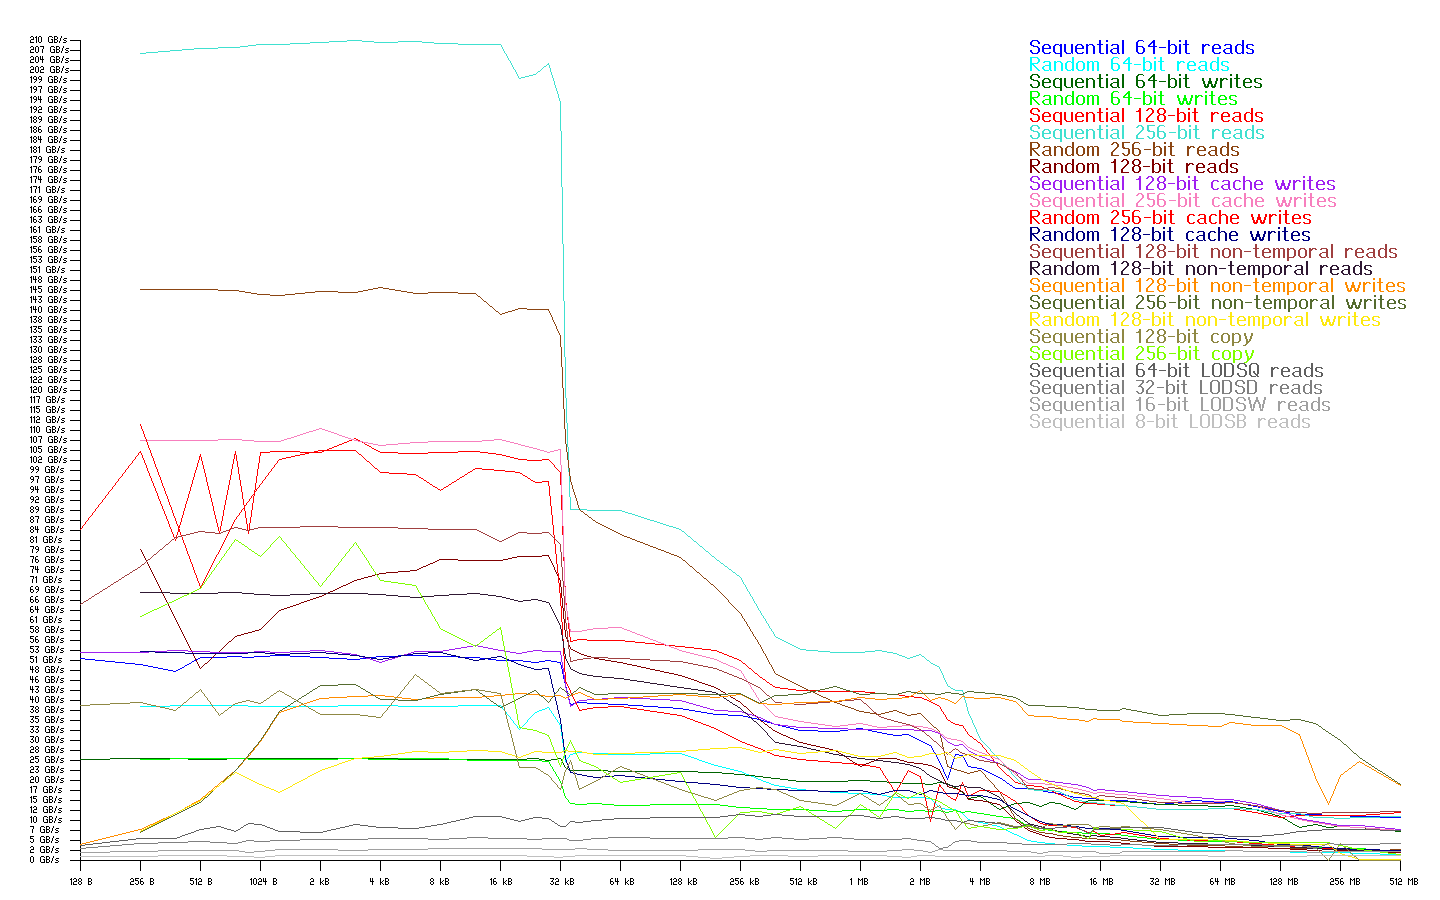
\includegraphics[width=0.6 \textwidth]{./bandwidth.png}	
	\caption{Results from the Docker bandwidth test showing bandwidth as a function of problem size for a Macbook Pro.}
\end{figure}

From this bandwidth test, we are able to estimate the size of each cache of this machine. The first feature that we notice in Figure \ref{fig:bandwidth} is a very significant drop in bandwidth then a plateau around 32 kB which suggests that the size of the L1 cache is approximately 32 kB since for problem sizes larger than than 32 kB, the processor must access data from another cache which reduces the bandwidth since other caches and memory are further away. The next feature that we notice is another drop and plateau in bandwidth that is a bit less dramatic than the previous drop and the plateau beginning around 256 kB suggesting that the L2 cache is approximately 256 kB. Finally, there is one more prominent drop and plateau in bandwidth with the plateau starting around 6 MB which suggests that the L3 cache is approximately 6 MB. After this test, the size of each cache was looked up from specification using the command "/usr/sbin/sysctl -a" resulting in seeing that the L1 cache has a size of 32768 bytes which is very close to the estimated 32 kB size, this information was found on a stack overflow post (https://stackoverflow.com/questions/5446134/determine-values-of-several-system-variables-in-the-terminal-in-a-mac
). The L2 cache had a size of 262144 bytes which is also very close to the estimated 256 kB size. Finally we see that the L3 cache has a size of 6291456 bytes which is also close to the estimated 6 MB seen in the experiment. Now that we know the size of the caches and their approximate bandwidths we could construct a roofline model for this machine. However, we will construct a roofline model using the Docker image provided. The roofline model program gives the results shown in Figure \ref{fig:roofline}. 

\begin{figure}[H]
	\centering
	\label{fig:roofline}
	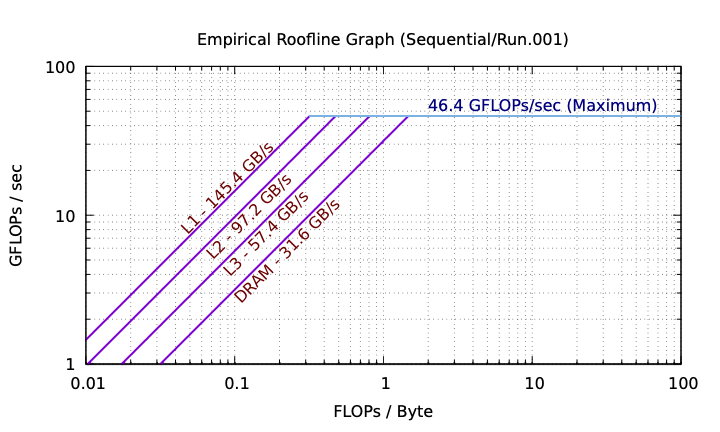
\includegraphics[width=0.7 \textwidth]{./roofline.png}	
	\caption{Roofline model for the Macbook pro used in this project.}
\end{figure}

From this roofline model shown in Figure \ref{fig:roofline} that the maximum performance of this computer is 46.4 GFLOPs/sec. From this figure we can also see that the L1 cache has a bandwidth of 145.4 GB/s, the L2 cache has a bandwidth of 97.2 GB/s, the L3 cache has a bandwidth of 57.4 GB/s and finally the dynamic random access memory (DRAM) has a bandwidth of 31.6 GB/s. When looking at Figure \ref{fig:bandwidth} above, we see that the bandwidths that were measured are generally lower than the maximum bandwidth of the L1 cache within the L1 cache regime (less than 32 kB) which could be due to other aspects of accessing memory. The Random 256-bit read had a measured bandwidth that was very close to the L1 cache bandwidth of 145.4 GB/s. The Random 64-bit read also had a much higher bandwidth of around 210 GB/s which is unexpected and could be due to other optimizations in the system. Using the clock speed of the CPU and the maximum GFLOP rate we can compute the maximum number of double precision floating point operations per clock cycle as in Equation \ref{eqn:floppercycle}. 
\begin{equation}
	\label{eqn:floppercycle}
	\frac{FLOPs}{cycle} = \frac{GFLOPs}{sec} * \frac{1}{Clock speed}
\end{equation}

Using this equation we estimate the number of double precision floating point operations per cycle to be approximately 20.2 flops/cycle. The hardware capabilities that allow for multiple flops per clock cycle are the vectorized registers in the CPU. As we saw from the cpuinfo583.cpp program, this computer supports SSE, AVX and AVX2 SIMD instruction sets as well as the fused multiply add(FMA) instruction set which implies that it has the hardware capability. If the FMA contributes a factor of two, SSE contrbutes a factor of two and AVX/AVX2 contributes a factor of four that would suggest we could get 16 flops/cycle and there could be other SIMD registers that were not listed that could be contributing to the computed 20.2 flops/cycle. 

% Section 2 - Improvements in Performance from correct usage of hierarchical memory
\section{Improvements in Performance from Better Usage of Hierarchical Memory}

As a baseline problem to use, we are interested in analyzing how we can get maximum performance out of the problem stated in Equation \ref{eqn:multtrans}. 
\begin{equation}
	\label{eqn:multtrans}
	C = A \times B^T
\end{equation}

This problem can be solved using many different algorithms that employ the use of techniques such as hoisting, blocking, tiling and others to improve the performance of this computation since this a computation ubiquitous to many fields of scientific computing. Using a few different algorithms to compute this matrix-matrix product for various problem sizes, we see the results in Appendix \ref{appendix:mmult-0}. Here we see that the transpose multiplications generally have higher performance by factors of up to three times higher performance than the matrix-matrix multiplications. This disparity between the two is most likely due to how the data is ordered and accessed through each loop and the time that it takes to access the data. The next step in understanding how to get the same performance out of the matrix-matrix multiply that we see with the matrix-transpose multiply is to understand more about loop ordering. In order to compute this matrix-matrix product we use three nested for loops with indices "i" for rows, "j" for columns and "k" for slabs. We now can rewrite algorithms for computing the matrix multiplications using different loop orderings and the associated performance. The results from this experiment are shown in Appendix \ref{appendix:mmult-1}. The best performing loop ordering was "ikj", the second best was "kij"while the two worst loop orderings were "kij" and "jki" as seen in Appendix \ref{appendix:mmult-1}. In order to better understand the differences between the loop orderings we must understand better how data is stored and accessed in memory. For the matrix data class that we have used in this class so far, the matrices are row-ordered which means that the elements in each row are store next to each other in memory. For the "ijk" ordering case, we can see one iteration of this loop in Figure \ref{fig:ijk} as provided through the problem assignment. 

\begin{figure}[H]
	\centering
	\label{fig:ijk}
	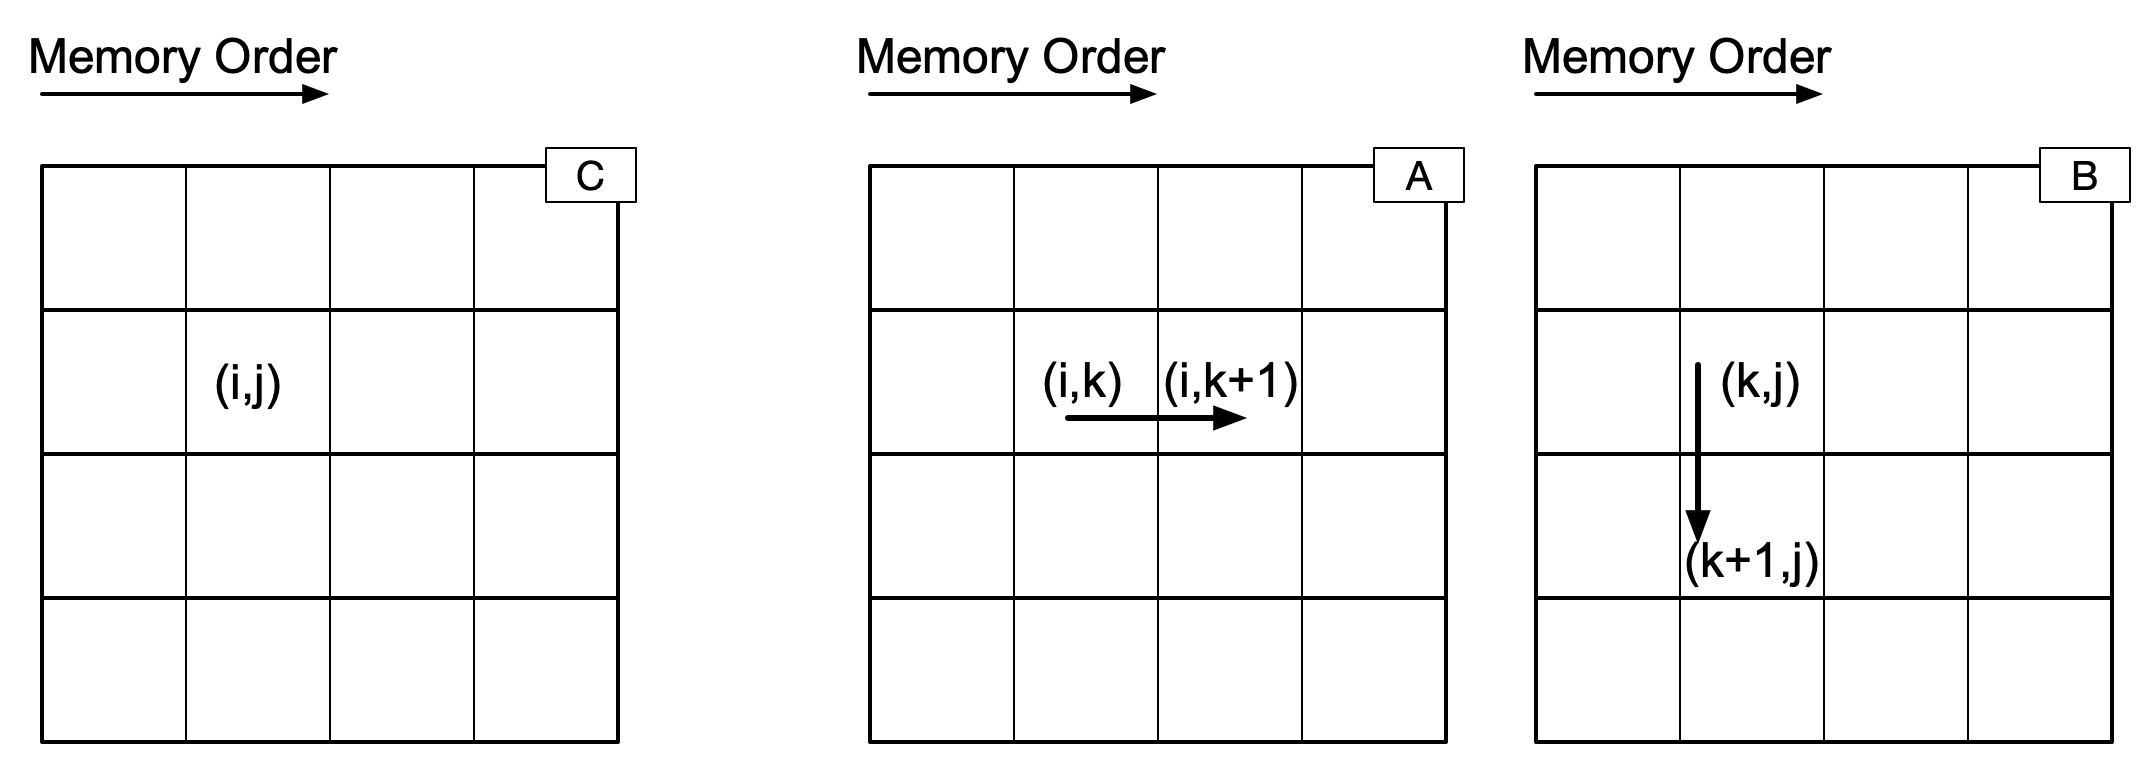
\includegraphics[width=0.7 \textwidth]{./ijk.png}	
	\caption{Graphic of one iteration of the inner loop for the "ijk" ordered matrix multiplication as provided in the problem assignment.}
\end{figure}


As we see in the graphic in Figure \ref{fig:ijk} we see that for each inner loop indexed with 'k' the value in matrix A can be easily accessed with the next value in memory being the next value to compute with while the value in matrix B is an entire row away and is out of order in memory. Now that we understand this, we have some more insight into why the "ikj" ordering gave the highest performance.The "ikj" ordering gave the highest performance since each inner loop iteration only the value of matrix B needed to be accessed while the value of A remained the same throughout so this ordering reduces the need to access two values from memory in each loop to only accessing one value for each loop. The "ikj" ordering also takes advantage of the row-ordered memory so each inner loop is moving to the next column which is the next element in a row and therefore the next closest element in memory so we can improve the locality of the data by using this loop ordering. When we look at the matrix transpose multiplication the difference between the zero optimization case and the first optimized case is that we "hoisted" the value C(i,j) out of the inner loop to the intermediate loop. The data access pattern for the matrix multiplication in "ijk" ordering will consist of accessing C(i,j), A(i,k) and B(j,k) at the step (i,j,k) then at the next step A(i, k+1) and B(j, k+1) will be accessed. This is advantageous since both values are stored next in memory since we move over a column in the same row for both matrices making it the fastest data access time.  When using "ijk" loop ordering, it is very beneficial to "hoist" C(i,j) out of the inner loop since this reduces the amount of data access in each iteration from three data accesses to only two. 

Now using some of these techniques of data access patterns we can optimize the matrix multiplication algorithms that we examined earlier. The difference between the second optimization and third optimization matrix multiplication algorithms is that the second optimization includes "hoisting" and "tiling" while the third optimization includes both the previous optimizations as well as rearranging the loop ordering to improve the memory access by switching to an "ikj" ordering. The best performance achieved by any of the multiplication algorithms was multiplication three after updating the loop ordering to "ikj" which resulted in a performance of 23.95 GFLOPs/sec with a problem size of 128. We can compare this performance to the bandwidth and roofline models predicted by computing the arithmetic intensity for this algorithm. We expect the arithmetic intensity of this algorithm to be 0.125 since in the inner most loop there are 8 float values accessed meaning 64 bytes of data being operated on and there are 8 operations resulting in an arithmetic intensity of 8/64 = 0.125. Since this problem also had a size of 128 the total data in the problem was approximately 4 MB and therefore it would fit in the L3 cache. Using the roofline model, we see that with this arithmetic intensity we expect to see a performance of approximately 20 GFLOPs/sec if the whole problem were in the L1 cache which is not expected due to its size. However, since there are vectorizations in the CPU which we do expect to have as discussed previously we could expect to see higher performance as we do. 

% Section - Array of Structure or Structure of Arrays 
\section{Array of Structures or Structures of Arrays}
Digital colored pictures are represented as a three dimensional structure where each pixel has three values to represent red, green and blue to represent the color of a pixel. The goal of this section is to understand what the best method of storing and accessing this data is whether we should store the values as a structure of arrays or as an array of structures. We will test the performance for three images with blurring functions to determine what the best way to store and access information is. The best blurring algorithm of the structure of arrays was the "outer" algorithm while the best performance for the array of structures was also "outer" and this was the same for the tensor where the "outer" algorithm gave the highest performance. The "outer" blurring kernel had the highest performance since the inner most loop was a "j" index so each column was being looped over in a row and since these data structures have row-major ordering the next element in a row is also the next element in memory which reduces the time spent accessing memory and thus improves performance. The blurring algorithm that had the best performance overall was the structure of arrays - outer 
	algorithm which had the best performance since it had "j" indexing as the inner most loop thus improving the data access and the structure of arrays also had the smallest innermost loop with only three elements which reduced the need for data access and therefore improved the performance of this algorithm. 


%% References
%\printbibliography

% Appendices
\begin{appendices}

% first log file
\section{mmult\_ps3.log}
\label{appendix:mmult-ps3} 
The values for this appendix are on the following page. 
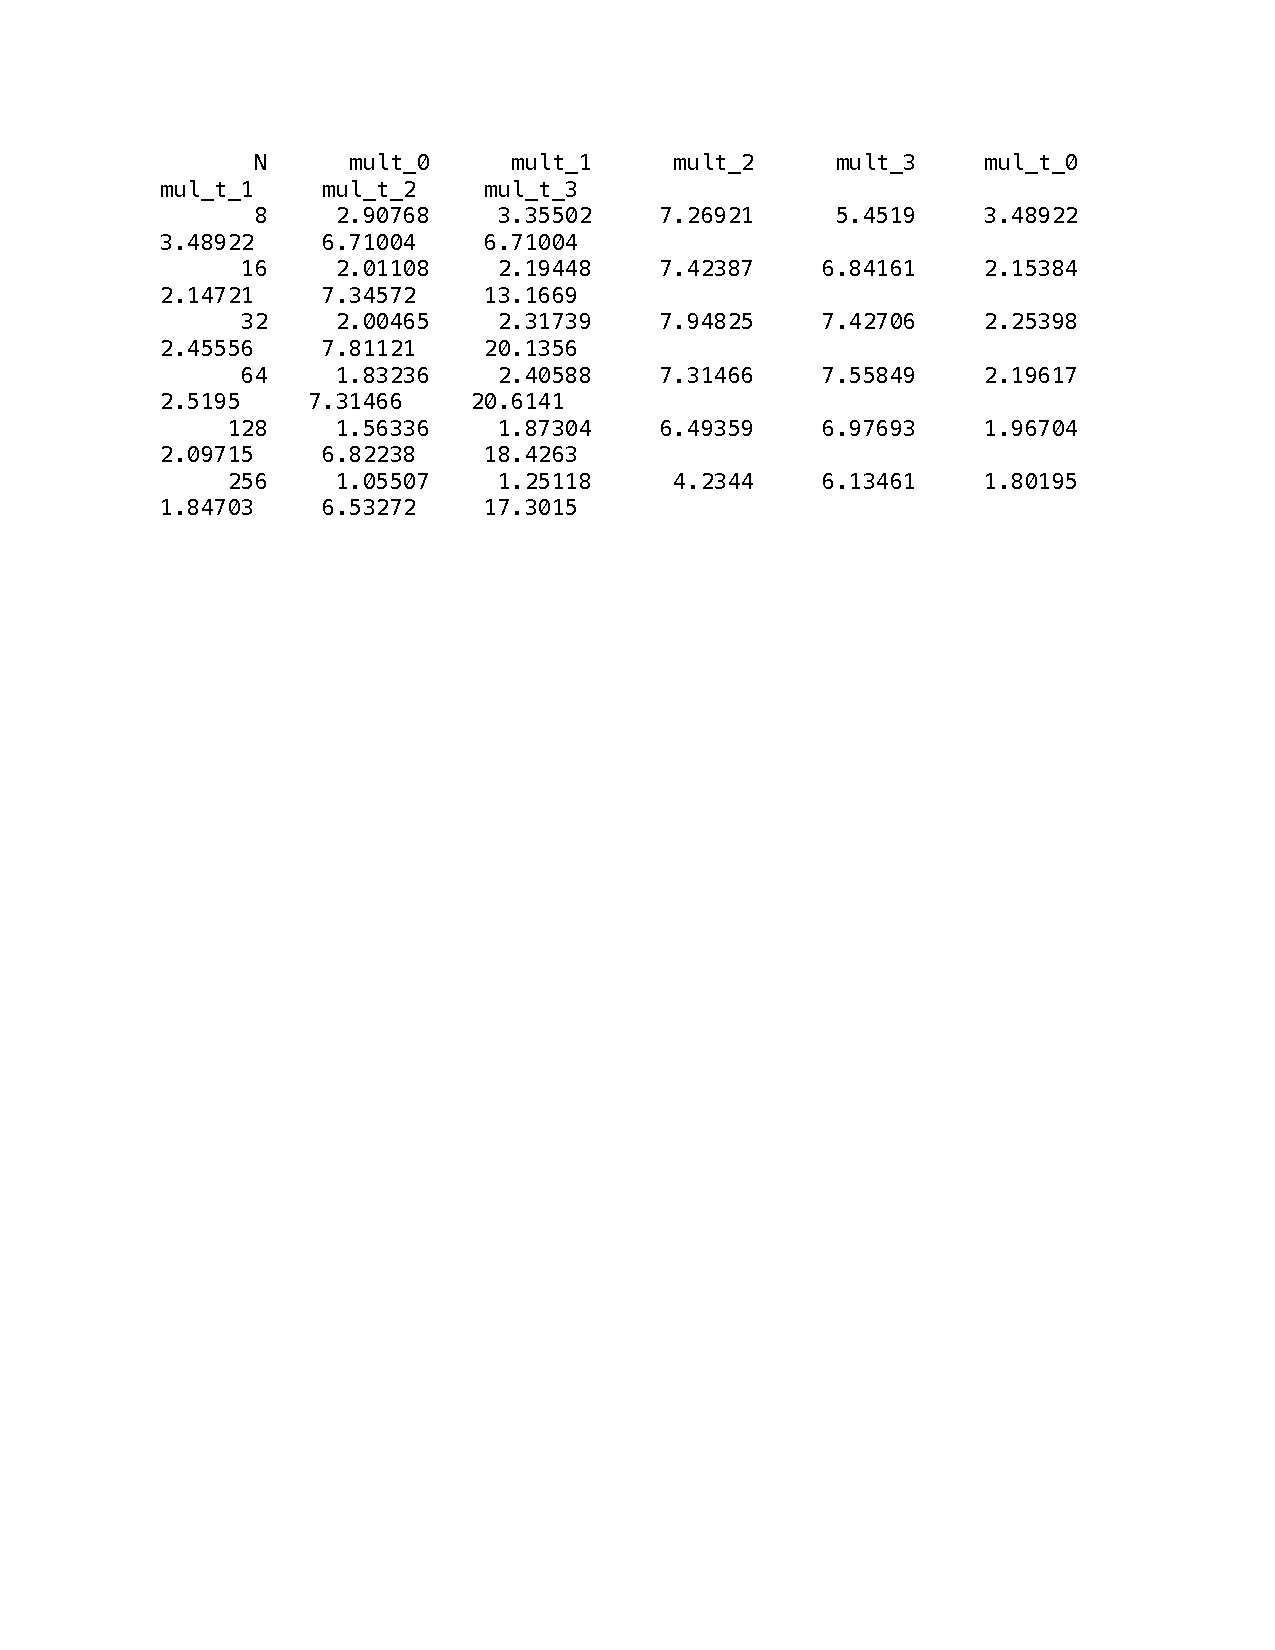
\includepdf[pages=-]{./mmult_ps3.pdf}

% Second log file
\section{mmult\_0.log}
\label{appendix:mmult-0} 
The values for this appendix are on the following page. 
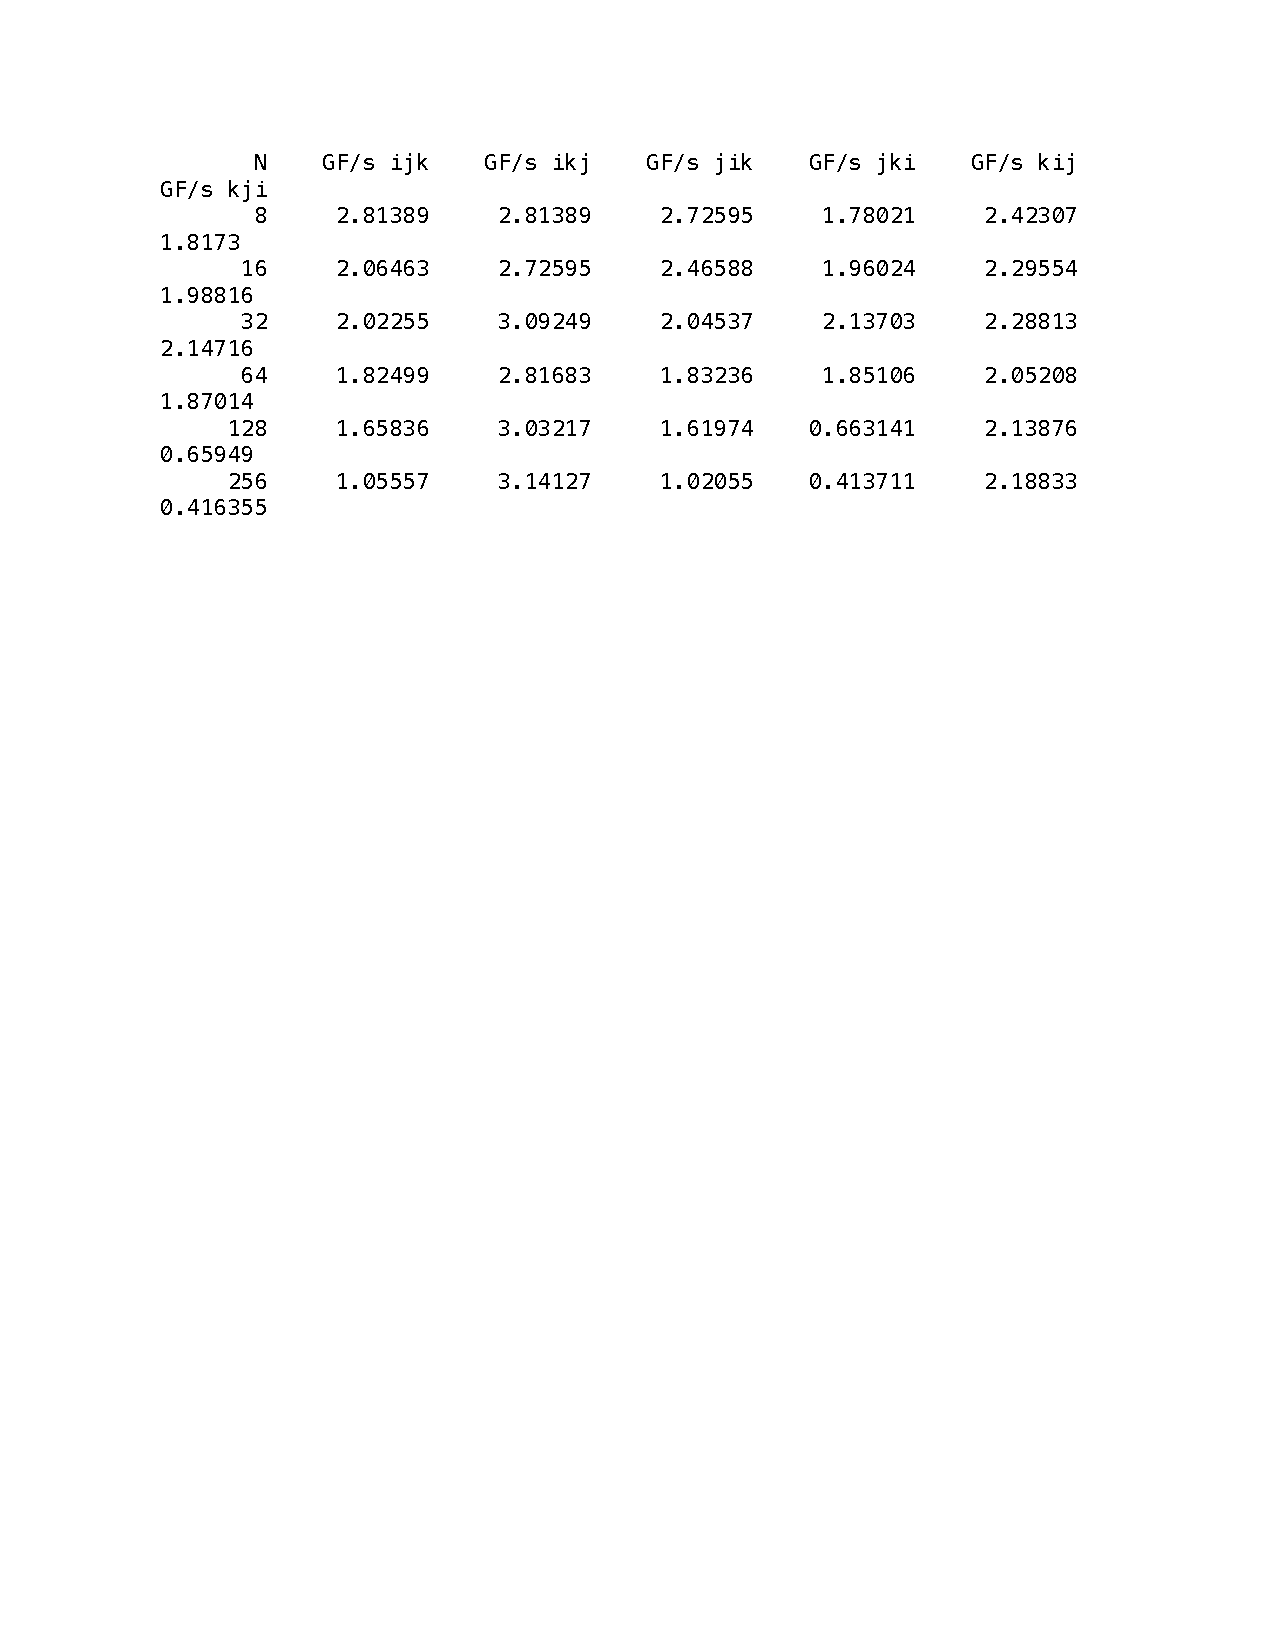
\includepdf[pages=-]{./mmult_0.pdf}

% Third log file
\section{mmult\_1.log}
\label{appendix:mmult-1} 
The values for this appendix are on the following page. 
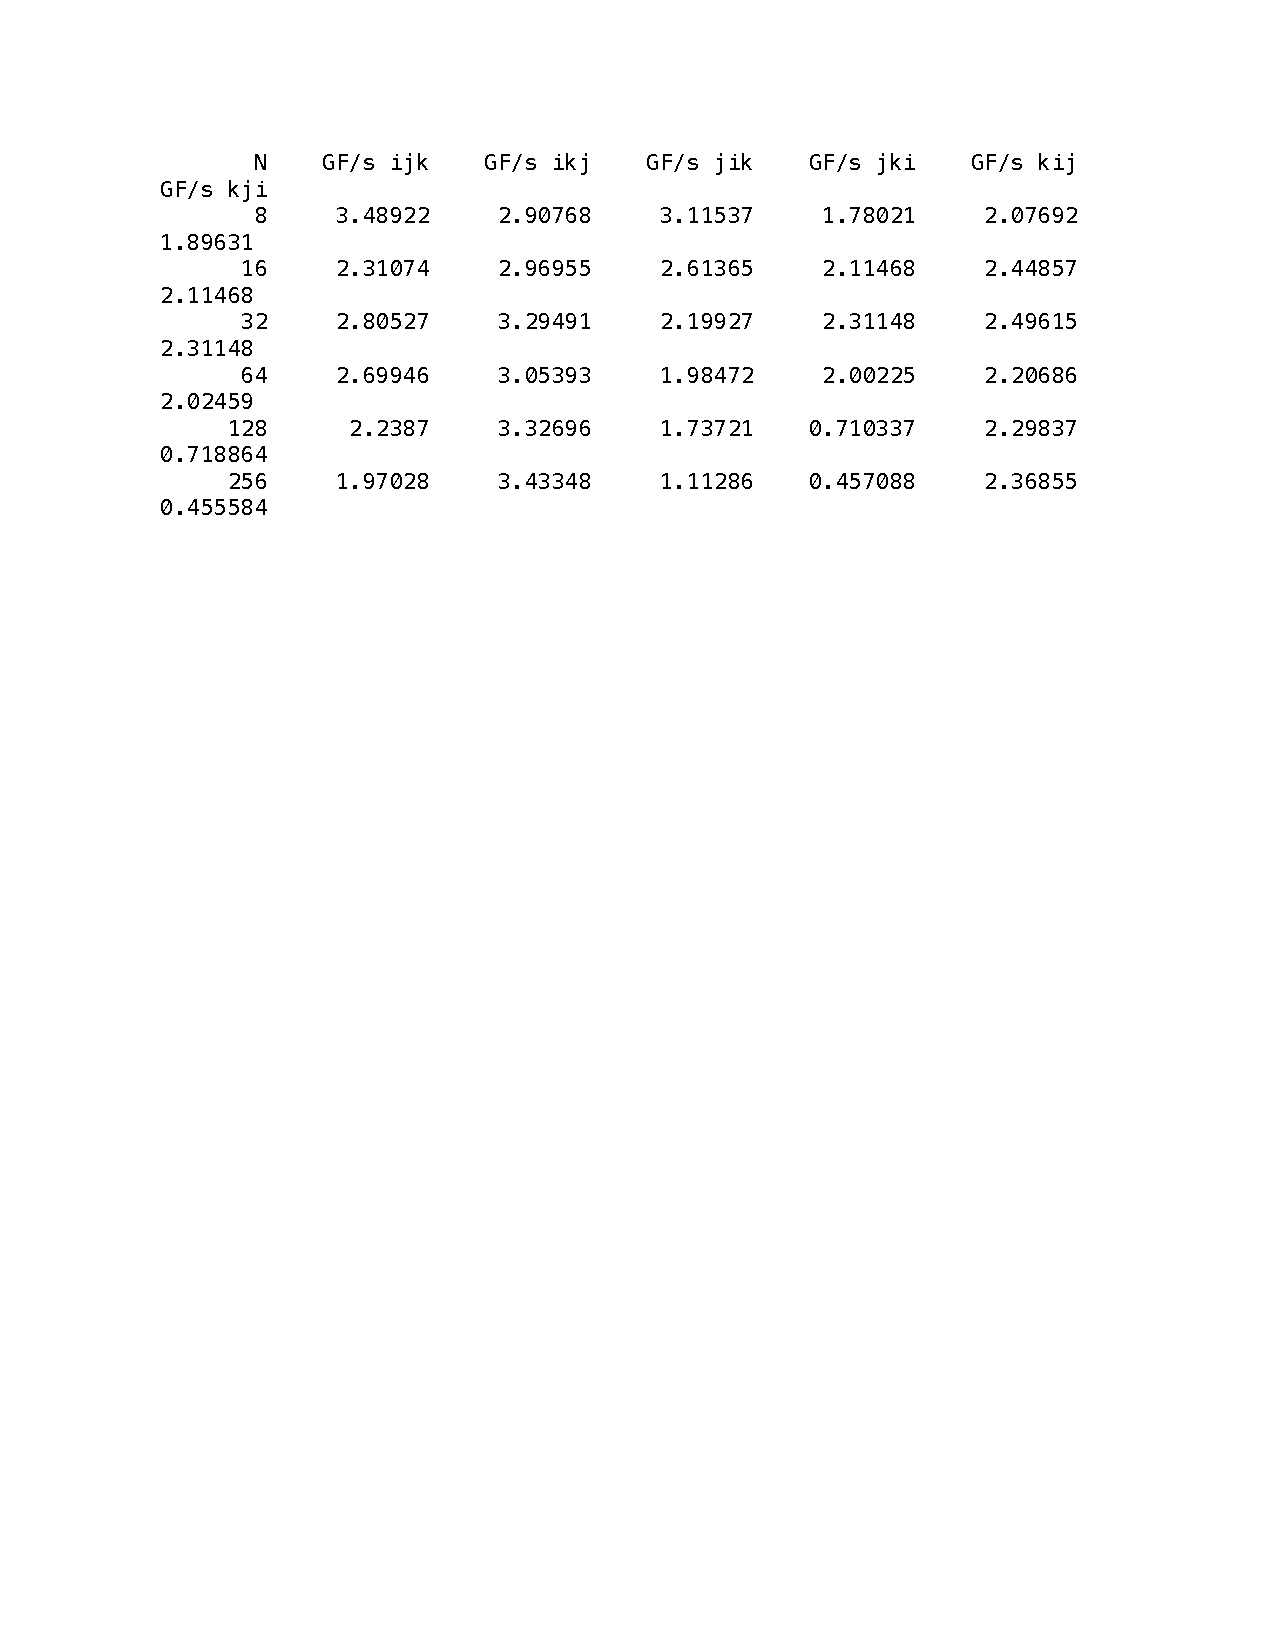
\includepdf[pages=-]{./mult_1.pdf}

% Fourth log file
\section{mmult\_2.log}
\label{appendix:mmult-2} 
The values for this appendix are on the following page. 
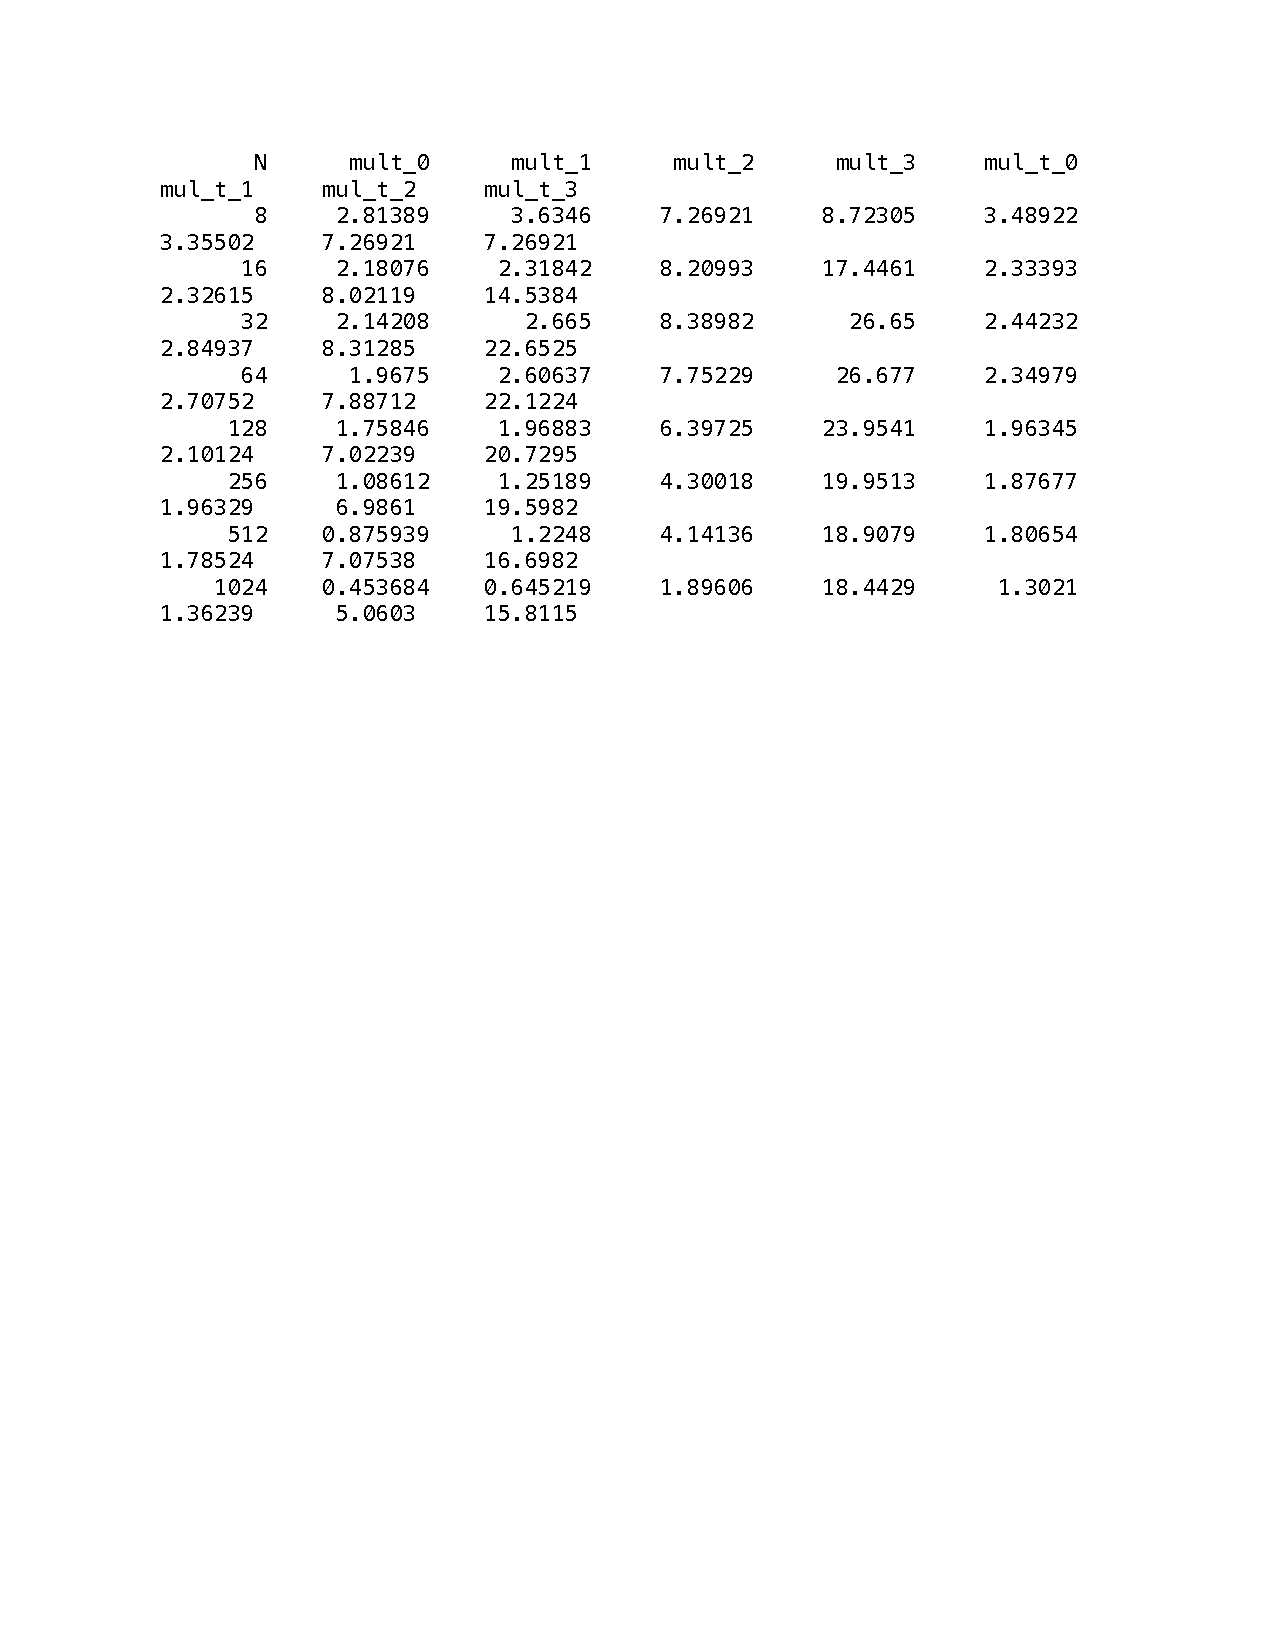
\includepdf[pages=-]{./mult_2.pdf}

\end{appendices}


\end{document}
